% ---------------------------------------------------------------------------
% Figura F2 — catálogo de sujetos.  Bloque listo para pegar en main.tex.
% NO insertado por la unidad: la inserción es de la autora.
%
% Ubicación sugerida: capítulo del esquema, §3.4, donde la prosa presenta el
% catálogo de sujetos y la cadena Sujetos -> ... -> Bancos comerciales.
%
% \includegraphics VA SIN EXTENSIÓN a propósito: pdflatex resuelve por su
% orden por omisión (.pdf antes que .png) y toma figura_catalogo_sujetos.pdf,
% el vectorial, con el texto como texto y sin depender de la resolución.  El
% PNG queda de respaldo y solo se usa si el PDF no está.  F1 y F1b, en
% cambio, llevan .png explícito.
%
% Sobre [H] y \linewidth: la figura mide 150 x 134,1 mm y su tipografía queda
% en 8,7 pt (etiquetas) y 8,1 pt (subtítulos, rótulos y leyenda).  Con
% width=0.85\linewidth —el ancho de F1 y F1b— bajaría a 114 mm de alto, pero
% la tipografía caería a 7,4 / 6,9 pt, por debajo del piso de 8 pt: por eso
% la figura va a ancho pleno.
%
% El epígrafe absorbe lo que se sacó de las cajas para ganar tipografía: los
% nombres desplegados de las dos instancias y la procedencia de la norma y
% del rol.  Con él, el bloque ocupa del orden de 194 a 199 mm de los 257 mm
% de caja de texto (a4 menos los márgenes de 2 cm de main.tex:9): cabe con
% [H] junto al párrafo que lo llama y deja unos 60 mm de texto en esa página.
% ESTIMACIÓN NO VERIFICADA por compilación — no hay LaTeX en el entorno donde
% se generó la figura, así que conviene mirar la primera corrida.
% ---------------------------------------------------------------------------
\begin{figure}[H]
  \centering
  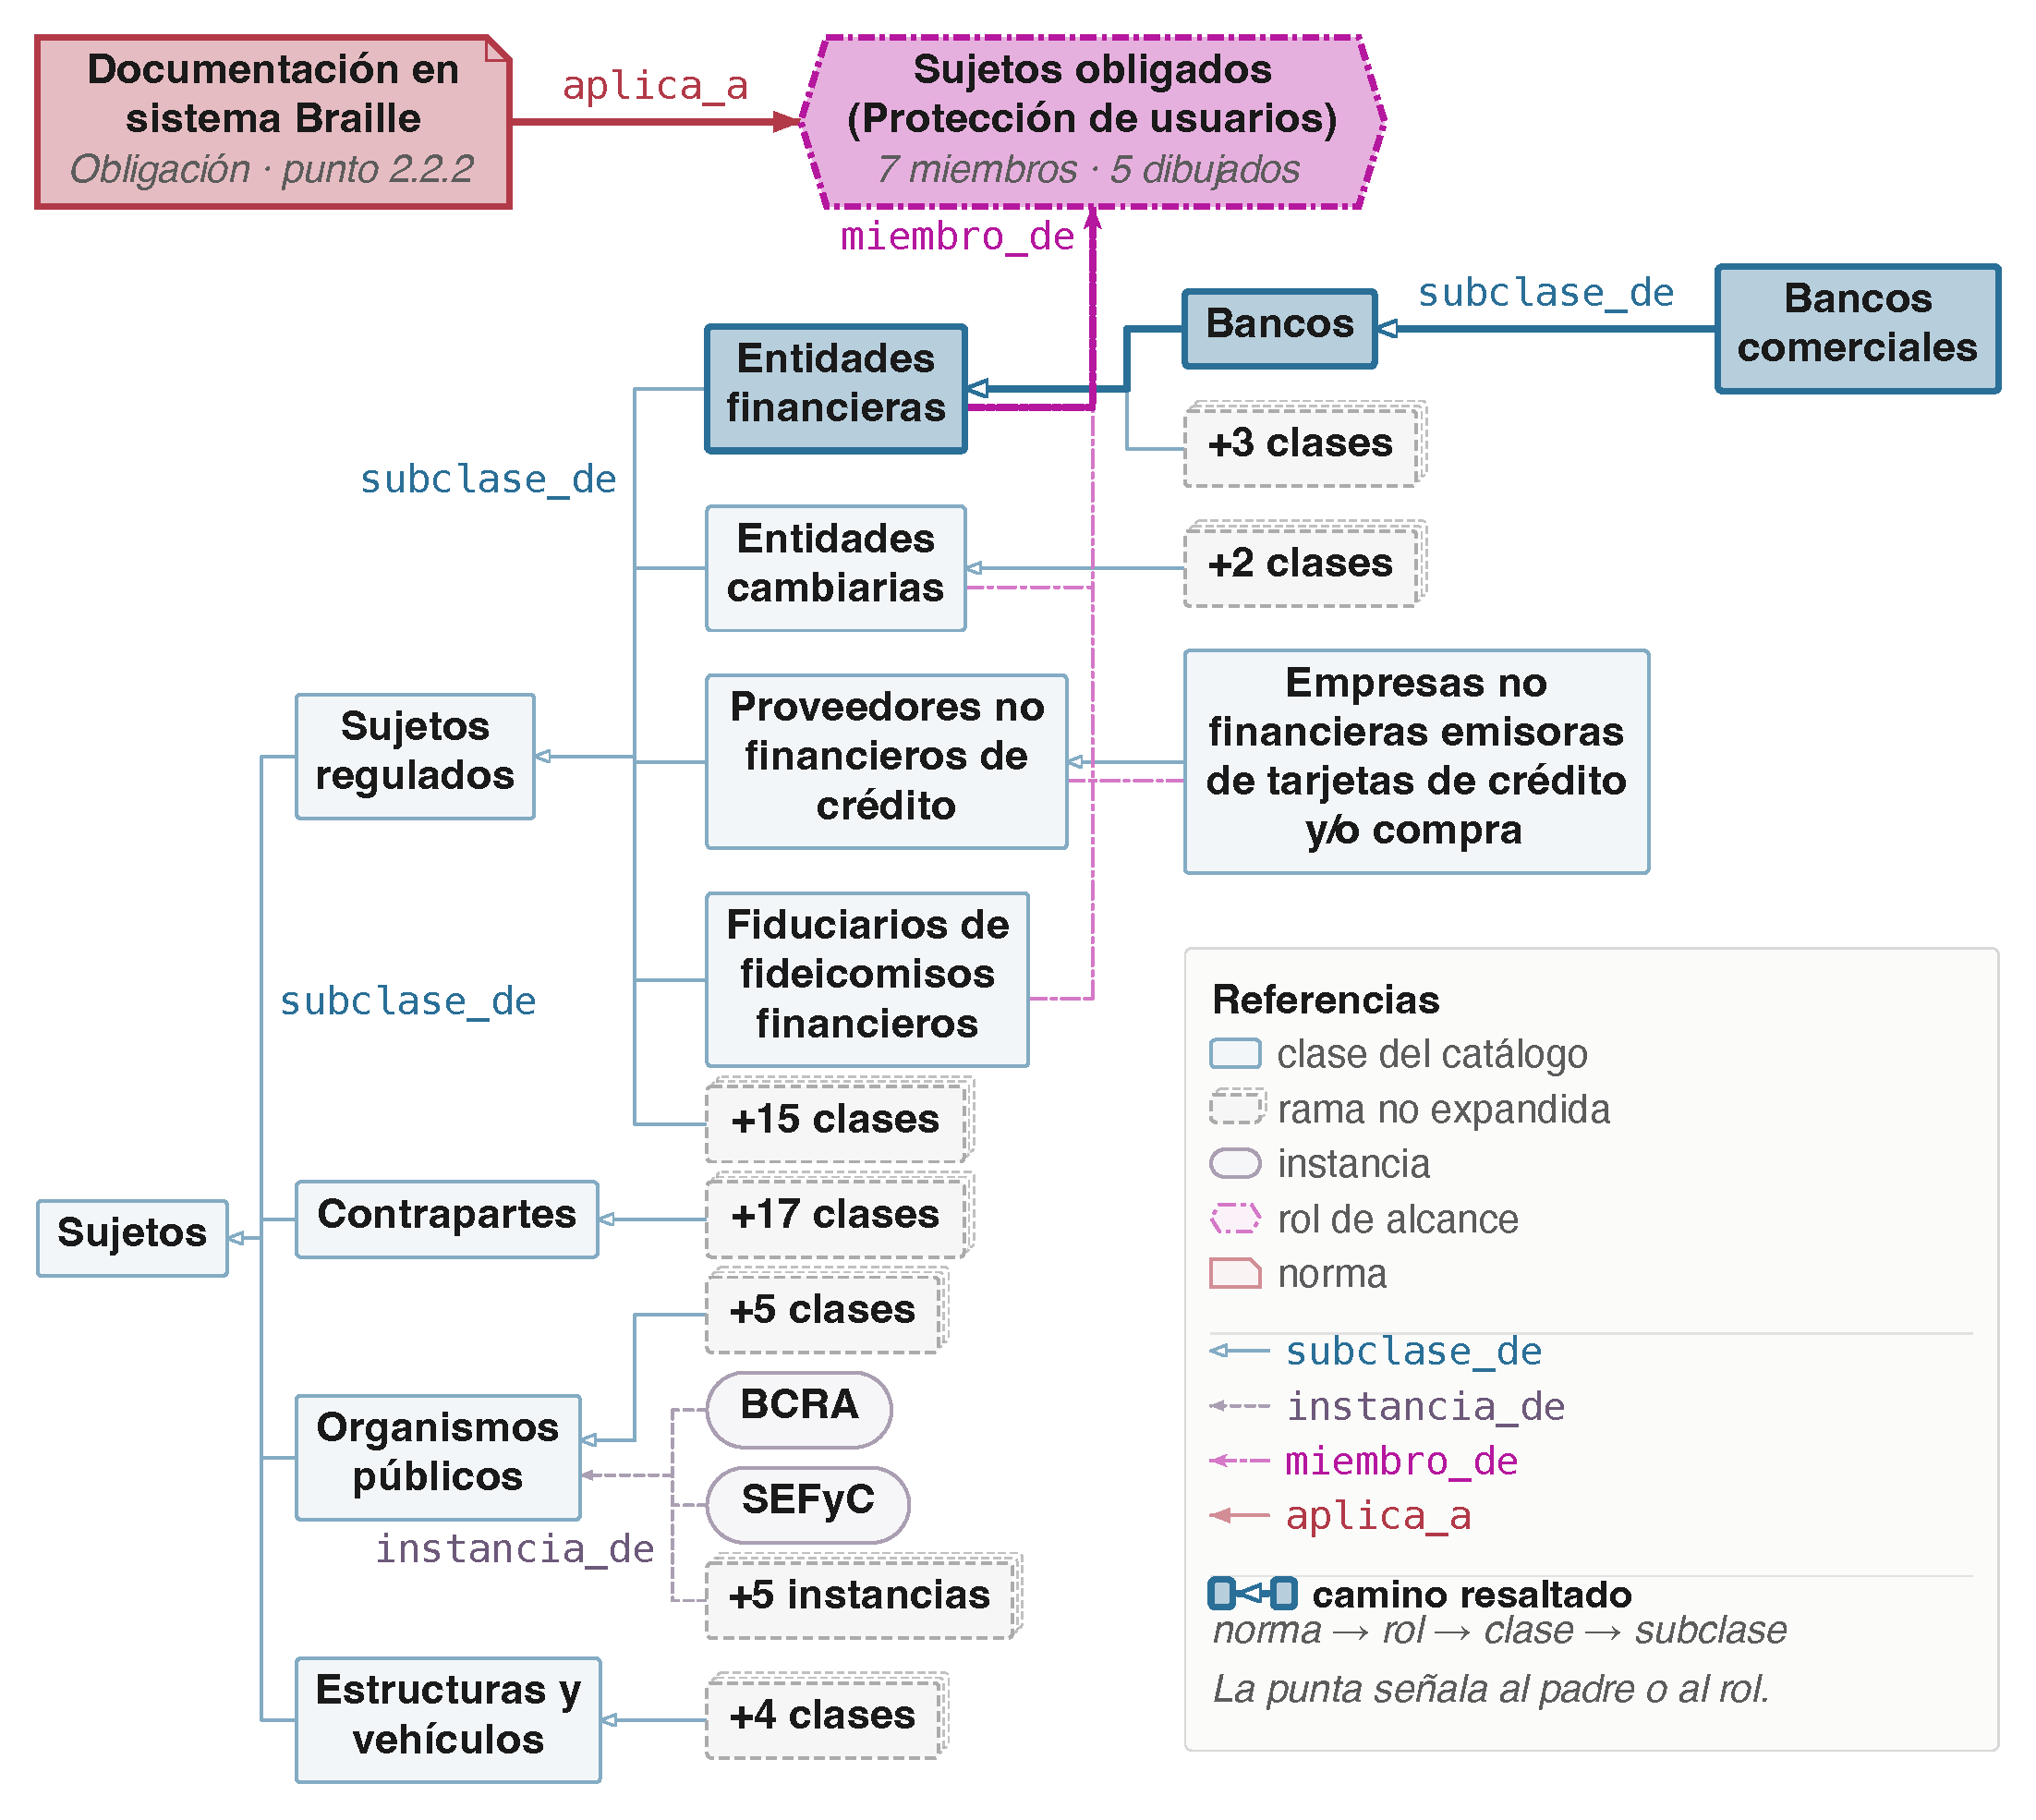
\includegraphics[width=\linewidth]{figuras/figura_catalogo_sujetos}
  \caption[El catálogo de sujetos]{El catálogo de sujetos. Las 58 clases
    forman un árbol único: la figura dibuja doce y colapsa las 46 restantes
    en nodos que declaran cuántas contienen. En trazo grueso, el camino que
    esta subsección recorre: la obligación de ofrecer documentación en
    sistema Braille (punto 2.2.2 del texto ordenado de protección de los
    usuarios) no nombra a ninguna clase, sino que apunta con
    \texttt{aplica\_a} al rol de alcance del punto 1.1.2; las clases
    declaran su pertenencia con \texttt{miembro\_de}, y de ahí el árbol
    baja hasta los bancos comerciales, que la norma nunca menciona. El rol
    tiene siete miembros y se dibujan cinco. Las instancias van por su sigla:
    BCRA, el Banco Central de la República Argentina, y SEFyC, la
    Superintendencia de Entidades Financieras y Cambiarias.}
  \label{fig:catalogo}
\end{figure}
